\renewcommand{\theequation}{\theenumi}
\renewcommand{\thefigure}{\theenumi}
\renewcommand{\thetable}{\theenumi}
\begin{enumerate}[label=\thesection.\arabic*.,ref=\thesection.\theenumi]
\numberwithin{equation}{enumi}
\numberwithin{figure}{enumi}
\numberwithin{table}{enumi}


\item Let  $X\in \{ 0,1 \}$ and $Y\in \{ 0,1 \}$ be two independent binary random variables. If $\pr{X=0}$ = p and  $\pr{Y=0}$ = q, then $\pr{X+Y \geqslant 1}$) is equal to 
\begin{enumerate}
\item $pq+(1-p)(1-q)$ 
\item  $pq$    
\item $p(1-q)$ 
\item  $1-pq$  
\end{enumerate}
%
\solution
%
%From the given information, 
\begin{align}
    p_{X}(n) &= 
\begin{cases}
p & n=0
\\
1-p & n=1
\end{cases}\label{sum/1/1}
\\
p_{Y}(n) &= 
\begin{cases}
q & n=0
\\
1-q & n=1
\end{cases}\label{sum/1/2}
\end{align}
%
  The characteristic functions of $X$ and $Y$ are 
%
\begin{align}
\phi_X(z)&=\mean{z^{-X}} =  p+(1-p)z^{-1}
\\
\phi_Y(z)&= q+(1-q)z^{-1}
\end{align}
and the CF of $  Z=X+Y$ is 
\begin{align}
\phi_{X+Y}(z)&=\mean{z^{-(X+Y)}} \\
               &=\phi_X(z)\times \phi_Y(z)
               \\
  & =\sbrak{p+(1-p)z^{-1}}\sbrak{q+(1-q)z^{-1}}
  \end{align}
  \begin{multline}
\implies \phi_{Z}(z) = pq+(p+q-2pq)z^{-1}\\
  +(1-p)(1-q)z^{-2}
\end{multline}
yielding 
%   From equation \eqref{sum/1/1}, we get\\
%     The pmf of Z is 
\begin{align}
    p_{Z}(n) = 
\begin{cases}
pq & n=0
\\
p+q-2pq & n=1\\
(1-p)(1-q) & n=2
\end{cases}\label{sum/1/3}
\end{align}
Thus, 
\begin{align}
    \pr{X+Y\geq1} = 1 - \pr{Z<1}= 1-pq   
\end{align}
%
\item Two independent random variables $X$ and $Y$ are uniformly distributed in the interval $\sbrak{-1,1}$. The probability that $\max \brak{X,Y}$ is less than $\dfrac{1}{2}$ is 
\begin{multicols}{4}
\begin{enumerate}
\item $\dfrac{3}{4}$
\item $\dfrac{9}{16}$
\item $\dfrac{1}{4}$
\item $\dfrac{2}{3}$
\end{enumerate}
\end{multicols}
\solution
%
%%
The  CDF of the X is 
 \begin{align}
 F_{X}(x)=\pr{ X<x }= \int _{-1}^{x} f_{X}(x) dx\\
 = \int _{-1}^{x} \dfrac{1}{2} dx= \dfrac{1}{2} \left( x-(-1) \right) = \dfrac{1}{2}( x+1) 
 \intertext{so} F_{X}(x)=\begin{cases}
 0   &   x<-1\\
 \dfrac{1}{2} (x+1) &   -1<x<1\\
 1  &   x>1 
 \end{cases}
  \label{indep/2/eq:9}
 \end{align}
$\because X, Y$ are independent,
 \begin{align}
 \pr{\max \brak{X,Y} < \dfrac{1}{2}}&= \pr{X<\dfrac{1}{2},  Y<\dfrac{1}{2} }
 \\
 & = \pr{ X<\dfrac{1}{2} } \times  \pr{Y<\dfrac{1}{2} }
 \label{indep/2/eq:7}
\\ 
& =\sbrak{F_{X}\left(\dfrac{1}{2} \right)}^2
\\
&= \dfrac{9}{16}
\end{align} 
upon substituting from   \eqref{indep/2/eq:9}.
So option 2 is correct answer 
%
\item Suppose that $X_1,X_2,X_3,...,X_{10}$ are i.i.d, N(0,1). Which of the following statements are correct ?
\begin{enumerate}[label = (\Alph*)]
    \item $\pr{X_1>X_2+X_3+...+X_{10}}=\frac{1}{2}$
    \item $\pr{X_1>X_2X_3...X_{10}}=\frac{1}{2}$
    \item $\pr{\sin{X_1}>\sin{X_2}+\sin{X_3}+...+\sin{X_{10}}}=\frac{1}{2}$
    \item $\pr{\sin{X_1}>\sin({X_2+X_3+\ldots+X_{10}})}=\frac{1}{2}$
\end{enumerate}
\solution
%
\begin{lemma}
    If $X \sim \mathcal{N}(0,1)$ then $Y =-X$ also follows standard normal distribution.
\end{lemma}
\begin{proof}
\begin{align}
    P(Y \leq u) &= P(-X \leq u) \\
    &= P(X > -u) \\
    &= 1 - P(X \leq -u) \\
    &= 1 - (1 - P(X \leq u) \\
    &= P(X \leq u) 
\end{align}
As the distribution is symmetric, 
\begin{align}
 P(X\leq -u)=P(X\geq u)= 1-P(X\leq u)   
\end{align} 
\end{proof}
\begin{lemma}
    If $n$ is an even number and $g(x)$ is an odd function, then,
    \begin{enumerate}
        \item 
    \begin{multline}\label{indep/3/equality}
        \pr{g(X_1)>\sum_{k=2}^ng(X_k)} \\=
        \pr{g(X_1)<\sum_{k=2}^ng(X_k)} \\
        = \frac{1}{2}
    \end{multline}
    \item 
    \begin{multline}
        \pr{g(X_1)>\prod_{k=2}^ng(X_k)}\\=
        \pr{g(X_1)<\prod_{k=2}^ng(X_k)} = \frac{1}{2}
    \end{multline}
    
\end{enumerate}
\end{lemma}
\begin{proof}
\begin{enumerate}
\item 
\begin{multline}
    \pr{g(X_1)>\sum_{k=2}^ng(X_k)}\\=
    \pr{g(-X_1)<\sum_{k=2}^ng(-X_k)}\\=
    \pr{g(X_1)<\sum_{k=2}^ng(X_k)}
\end{multline}
%
As the cases
\begin{align}
    g(X_1)>\sum_{k=2}^ng(X_k)
\end{align}
and
\begin{align}
    {g(X_1)<\sum_{k=2}^ng(X_k)}
\end{align}
are complementary to each other, 
\begin{align}\label{indep/3/sum}
 \pr{g(X_1)>\sum_{k=2}^ng(X_k)}=\frac{1}{2}    
\end{align}
%
\item Similarly, 
\begin{multline}
    \pr{g(X_1)>\prod_{k=2}^ng(X_k)}\\=
    \pr{g(-X_1)<\prod_{k=2}^ng(-X_k)}\\=
    \pr{g(X_1)<\prod_{k=2}^ng(X_k)}
\end{multline}
As they follow the same distribution, the above expression is true. Thus we have
\begin{align}
    %\label{indep/3/equality}
    \pr{g(X_1)>\prod_{k=2}^ng(X_k)}=
    \pr{g(X_1)<\prod_{k=2}^ng(X_k)}
\end{align}
%
As the cases
\begin{align}
    g(X_1)>\prod_{k=2}^ng(X_k)
\end{align}
and
\begin{align}
    {g(X_1)<\prod_{k=2}^ng(X_k)}
\end{align}
are complementary to each other and from 
 \eqref{indep/3/equality} we have
\begin{align}\label{indep/3/prod}
 \pr{g(X_1)>\prod_{k=2}^ng(X_k)}=\frac{1}{2}    
\end{align}
\end{enumerate}
\begin{enumerate}[label = (\Alph*)]
    \item 
    From \eqref{indep/3/sum} , taking $g(x)=x$,
    \begin{align}
        \pr{X_1>X_2+...+X_{10}}=\frac{1}{2}
    \end{align}
\item
From \eqref{indep/3/prod} taking $g(x)=x$
        \begin{align}
         \pr{X_1>X_2X_3...X_{10}}=\frac{1}{2}   
        \end{align}
\item 
From \eqref{indep/3/sum} taking $g(x)=\sin{x}$
        \begin{align}
         \pr{\sin{X_1}>\sin{X_2}+...+\sin{X_{10}}}=\frac{1}{2}   
        \end{align}
\item \begin{multline}
        \pr{\sin{X_1}>\sin{(X_2+...+X_{10})}}\\=\pr{\sin{(-X_1)}<\sin{(-X_2-...-X_{10})}}\\
        =\pr{\sin{X_1}<\sin{(X_2+...+X_{10})}}
    \end{multline}
    As they follow the same distribution, the above expression is true.
    Thus we have
    \begin{multline} 
    \pr{\sin{X_1}>\sin{(X_2+...+X_{10}})}\\
        =\pr{\sin{X_1}<\sin{(X_2+...+X_{10}})}    
    \end{multline}
    Also, as $X_1$ is a continuous random variable
    \begin{align}
       \pr{\sin{X_1}=\sin{(X_2+...+X_{10})}}=0
    \end{align}
     As the cases
     \begin{align}
      {X_1>X_2+...+X_{10}}   
     \end{align}and 
     \begin{align}
         {X_1<X_2+...+X_{10}}
     \end{align}are complementary to each other 
        \begin{align}
         \pr{\sin{X_1}>\sin{(X_2+...+X_{10}})}=\frac{1}{2}   
        \end{align}
\end{enumerate}
\end{proof}

\item Which of the following conditions imply independence of the random variables $X$
and $Y$ ?
\begin{enumerate}
    \item  $\pr{X\ \mathop{>}\ a|Y\ \mathop{>}\ a} = \pr{X\ \mathop{>}\ a}\ \forall\ a\ \in\ \mathbb{R}$\\ 
    \item  $\pr{X\ \mathop{>}\ a|Y\ \mathop{<}\ b} = \pr{X\ \mathop{>}\ a}\ \forall\ a,\ b\ \in\ \mathbb{R}$\\ 
    \item  $X$ and $Y$ are uncorrelated.\\
    \item  $E[(X-a)(Y-b)] = E(X-a)\ E(Y-b)\ \forall\ a,\ b \in\ \mathbb{R}$\\
\end{enumerate}
%
\solution
%

\begin{definition}
    Two random variables $X$ and $Y$ are independent when the joint probability distribution of random variables is product of their individual probability distributions i.e for all sets A,B
    \begin{align}
        \label{indep/4/eq1} \pr{X\in A,Y \in B}=\pr{X \in A}\pr{Y \in B}
    \end{align}
    Alternatively, 
    \begin{align}
        \label{indep/4/eq1/cdf} F_{X,Y}\brak{a,b}=F_X\brak{a}F_Y\brak{b}
     \end{align}
  
\end{definition}
\begin{lemma}
From \eqref{indep/4/eq1/cdf}, it follows that 
\begin{align}
    \implies f_{X,Y}\brak{a,b}=f_X\brak{a}f_Y\brak{b}
    \label{indep/4/eq1/pdf}
\end{align}
\end{lemma}
\begin{proof}
    From \eqref{indep/4/eq1/cdf},
    \begin{align}
        \frac{\partial^2 F_{X,Y}\brak{a,b}}{\partial b \partial a}=\frac{\partial F_X\brak{a} }{\partial a}\frac{\partial F_Y\brak{b} }{\partial b} 
    \end{align}
    yielding     \eqref{indep/4/eq1/pdf}.
\end{proof}


\begin{enumerate}
     \item  From the given information, 
     \begin{align}
        \pr{X>a,Y>a} &=         \pr{X>a}\pr{Y>a}
        \\
        &= \sbrak{1-F_X\brak{a}}\sbrak{1-F_Y\brak{a}}
        \label{indep/4/eq1/sp/1}
     \end{align}
    \begin{multline}
\because \pr{X>a}-\pr{Y<a}\\=\pr{X>a,Y>a}+\pr{X>a,Y<a}\\-\pr{X>a,Y<a}-\pr{X<a,Y<a}, 
\\
\pr{X>a,Y>a} =         1-F_X\brak{a}-F_Y\brak{a}\\ +F_{X,Y}\brak{a,a}
    \end{multline}
which, upon substituting from         \eqref{indep/4/eq1/sp/1} yields
\begin{align}
\implies F_{X,Y}\brak{a,a}=F_X\brak{a}F_Y\brak{a}
\label{indep/4/eq1/sp}
\end{align}
which is a special case of \eqref{indep/4/eq1} for $b=a$.  The spectrum of conditions for independence is hence underrepresented. 
Thus, the given  condition does not imply independence of $X$ and $Y$.    
% \begin{example}
%     Consider two random variables $X$,$Y \in \{0,1,2\}$ with the probabilities of the ordered pairs \brak{X,Y} given in the Table\ref{indep/4/table1}.  The given
%     distribution satisfies 
% \end{example}
%     \begin{table}[!ht]
%      \centering
%      \resizebox{\columnwidth}{!}{
% \begin{tabular}{|l|c|c|c|}
%     \hline
%     \diagbox{$X$}{$Y$}&0&1&2\\ 
%     \hline
%      0&0.2&0.1 &0.1\\     \hline
%      1&0.2&0.1&0.05\\     \hline
%      2&0.1&0.1&0.05\\     \hline
%     \hline
%     \end{tabular}}
%     \caption{\pr{X,Y}}
%     \label{indep/4/table1}
%         \end{table}    
    
%     Case 1: $a<0$
%     \begin{align}
%         \pr{X>a|Y>a}=1=\pr{X>a}
%     \end{align}
%     Case 2: $0\leq a <1$
%     \begin{align}
%         \pr{X>a|Y>a}=\frac{\pr{X,Y>a}}{\pr{Y>a}}=\frac{0.3}{0.5}=0.6\\
%         \pr{X>a}=\pr{X=1}+\pr{X=2}=0.6
%     \end{align}
%     Case 3: $1\leq a <2$
%     \begin{align}
%         \pr{X>a|Y>a}=\frac{\pr{X,Y>a}}{\pr{Y>a}}=\frac{0.05}{0.2}=0.25\\
%         \pr{X>a}=\pr{X=2}=0.25
%     \end{align}
%     Case 4: $a\geq 2$
%     \begin{align}
%         \pr{X>a|Y>a}=\frac{\pr{X,Y>a}}{\pr{Y>a}}
%     \end{align}
%     is not defined as $\pr{Y>a}=0$.
%     In all the cases, $\pr{X>a|Y>a}=\pr{X>a}$ is true.
    
%     Consider,
%     \begin{align}
%         \pr{X=1,Y=2}=0.05
%     \end{align}
%     \begin{multline}
%         \pr{X=1}\pr{Y=2}=0.35\times0.2=0.7\\\neq\pr{X=1,Y=2}
%     \end{multline} 
%     Clearly, $X$ and $Y$ are not independent. 
    
     {\em Option 1 is incorrect}.
    
    \item From Bayes theorem,
    \begin{align}
        \pr{X>a|Y<b}&=\pr{X>a}
    \end{align}
    \begin{multline}
            \label{indep/4/eq3}
            \implies \pr{X>a,Y<b} \\ =\pr{X>a}\pr{Y<b}
        \end{multline}
    for all $a,b\in R$. 
    \begin{multline}
    \because     F_Y\brak{b}=\pr{X>a,Y<b} \\ +\pr{X<a,Y<b}, 
    \end{multline}
    \begin{multline}
    \pr{X>a,Y<b} \\= F_Y\brak{b}-F_{X,Y}\brak{a,b}
    \\
    \implies           F_Y\brak{b}-F_{X,Y}\brak{a,b} \\=\brak{1-F_X\brak{a}}F_Y\brak{b}\\
    \text{or, }
        F_{X,Y}\brak{a,b}=F_X\brak{a}F_Y\brak{b}
    \end{multline}
    upon substituting from  \eqref{indep/4/eq3} and simplifying.
     Thus, $X$ and $Y$ are independent. 
    
{\em Option 2 is correct}.
\item  We prove through a counterexample.
\begin{definition}
    Two random variables $X$ and $Y$ are uncorrelated if their covariance is zero, i.e., 
    \begin{align}
        \cov{X}{Y}=\mean{XY}-\mean{X}\mean{Y}=0
    \end{align}
\end{definition}
    % Uncorrelatedness does not imply independence.
    Let $X\sim U \sbrak{-1,1}$ be a uniformly distributed random variable such that 
    \begin{align}
        f_X\brak{x}=
        \begin{cases}
        \frac{1}{2} & -1\leq x \leq 1\\
        0 & otherwise
        \end{cases}\\
        \mean{X}=\int_{-1}^{1}x f\brak{x} dx=0
    \end{align}
    Let 
    \begin{align}
        Y=X^2.
    \end{align}
   so that  $X$ and $Y$ are dependent.  Then, 
    \begin{align}
        \cov{X}{Y}&=\mean{XY}-\mean{X}\mean{Y}\\
        &=\mean{X^3}-0\times \mean{Y}\\
        &=\int_{-1}^{1}x^3 f\brak{x} dx=0
    \end{align}
    $X$ and $Y$ are uncorrelated but not independent.
    
    {\em Option 3 is incorrect}
    
    \item Given that,
    \begin{align}
        \mean{\brak{X-a}\brak{Y-b}}=\mean{X-a}\mean{Y-b}
    \end{align}
    \begin{multline}
    \implies     \cov{X-a}{Y-b}=
    \\
        \mean{\brak{X-a}\brak{Y-b}}\\-\mean{X-a}\mean{Y-b}
    \end{multline}
    \begin{align}
        \text{or, } \cov{X-a}{Y-b}=0=\cov{X}{Y}
    \end{align}
    From option 3, it follows that $X$ and $Y$ are not necessarily independent.
    
    \textbf{Option 4 is incorrect.}
\end{enumerate}

%
\item Let X and Y be two independent and identically distributed (I.I.D) random variables uniformly distributed in (0,1). Let $Z = max(X,Y)$ and $W = min(X,Y)$ , then the probability that $[Z-W >\frac{1}{2}]$ is\\
\\(A) $\frac{1}{2}$\\
\\(B) $\frac{3}{4}$\\
\\(C) $\frac{1}{4}$\\
\\(D) $\frac{2}{3}$    
%
\solution

X and Y are two independent random variables. \\
Let
\begin{align}
    f_X\brak{x} &= \Pr\brak{X=x} \\
    f_Y\brak{y} &= \Pr\brak{Y=y}  \\
    f_V\brak{v} &= \Pr\brak{V=v}
\end{align}
be the probability densities of random variables X ,Y and V=X-Y.\\
The density for X is \\
\begin{align}
\label{june2018-50eq:_pdf_x}
f_{X}(x)  = 
\begin{cases}
1 & 0 \le x \le 1
\\
0 & otherwise
\end{cases}
\end{align}
We have ,
\begin{equation}
    V= X-Y \iff v= x- y \iff x = v+y
\end{equation}
The density of X can also be represented as,
\begin{align}
\label{june2018-50eq:pdf_x}
f_{X}(v+y)  = 
\begin{cases}
1 & 0 \le v+y \le 1
\\
0 & otherwise
\end{cases}
\end{align}
and the density of Y is,
\begin{align}
\label{june2018-50eq:pdf_y}
f_{Y}(y)  = 
\begin{cases}
1 & 0 \le y \le 1
\\
0 & otherwise
\end{cases}
\end{align}
The density of V i.e. $V=X-Y $ is given by the convolution of $f_X(-v)$ with $f_Y(v)$.
\begin{equation}
    f_V(v) =  \int_{- \infty}^{\infty} f_X(v+y)f_Y(y) \,dy 
\end{equation}
From \ref{june2018-50eq:pdf_x} and \ref{june2018-50eq:pdf_y} we have, \\
The integrand is 1 when,
\begin{align}
    0 \le y \le 1 \\
    0 \le v+y \le 1 \\
    -v \le y \le 1-v
\end{align}
and zero, otherwise. \\
Now when $-1 \le v \le 0$ we have, 
\begin{align}
    f_V(v) &=   \int_{-v}^{1} \,dy  \\
          &= (1 - (-v)) \\
          &= 1+v
\end{align}

For $0 \le v \le 1$ we have, 
\begin{align}
    f_V(v) &=   \int_{0}^{1-v} \,dy  \\
          &= (1-v - (0)) \\
          &= 1-v
\end{align}

Therefore the density of V is given by
\begin{align}
\label{june2018-50eq:pdf_v}
f_{V}(v)  = 
\begin{cases}
1+v & -1 \le v \le 0
\\
1-v & 0 < v \le 1
\\
0 & otherwise
\end{cases}
\end{align}

The plot for PDF of $V $ can be observed at figure \ref{june2018-50fig:The PDF of V}
\begin{figure}[!ht]
       \centering
    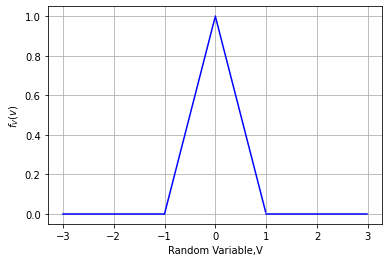
\includegraphics[width=\columnwidth] {solutions/2018/june/50/Assignment_3_Fig_1.png}
    \caption{The PDF of V}
    \label{june2018-50fig:The PDF of V}
\end{figure}

The CDF of V is defined as,
\begin{equation}
    F_V(v) = \Pr\brak{V \le v}
\end{equation}
Now for $ v \le 0 $,
 \begin{align}
    \Pr\brak{V\le v} &=  \int_{-\infty}^{v}f_{V}(v) \,dv  \\
          &=  \int_{-1}^{v} (1+v) \,dv  \\
          &=  \left(\dfrac{v^2}{2}+v \right) \Biggr|_{-1}^{v}  \\
          &=   \left(\left(\dfrac{v^2}{2}+v \right) - \left(\dfrac{1}{2} -1 \right)\right) \\
          &= \dfrac{v^2+2v +1}{2}
\end{align}
Similarly for $v \le 1$,
\begin{align}
    \Pr\brak{V\le v} &=  \int_{-\infty}^{v}f_{V}(v) \,dv  \\
          &=  \dfrac{1}{2} + \int_{0}^{v}(1-v)\,dz  \\
          &=  \dfrac{-v^2+2v+1}{2}
\end{align}

The CDF is as below: 
\begin{align}
\label{june2018-50eq:cdf_v}
F_{V}(v)  = 
\begin{cases}
0 & v < -1
\\
\dfrac{v^2+2v + 1}{2} &  v \le 0
\\
\dfrac{-v^2+2v+1}{2} &  v \le 1
\\
1 & v > 1
\end{cases}
\end{align}

The plot for CDF of $V $ can be observed at figure \ref{june2018-50fig:The CDF of V}\\

\begin{figure}[!ht]
       \centering
    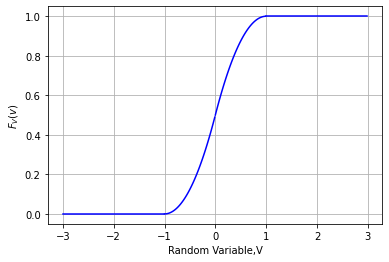
\includegraphics[width=\columnwidth] {solutions/2018/june/50/Assignment_3_Fig_2.png}
    \caption{The CDF of V}
    \label{june2018-50fig:The CDF of V}
\end{figure}

We need  $\pr{Z-W >\frac{1}{2}}$ where $Z = max(X,Y)$ and $W = min(X,Y)$. Now,

\begin{align}
\label{june2018-50eq:pdf_v}
Z-W  = 
\begin{cases}
X-Y & \text{for } X \geq Y
\\
Y-X & \text{for } X < Y
\end{cases}
\end{align}

Therefore,
\begin{align}
    \pr{Z-W >\frac{1}{2}} &= \pr{X-Y>\frac{1}{2},X \geq Y} \nonumber \\
    &+\pr{Y-X > \frac{1}{2}, X < Y}\\
    &= \pr{X-Y>\frac{1}{2}} +\pr{Y-X>\frac{1}{2}}\\
    &= \pr{V > \frac{1}{2}} + \pr{-V > \frac{1}{2}}\\
    &= 1 - \pr{V \leq \frac{1}{2}} + \pr{V < \frac{-1}{2}}\\
    &= 1-F_V(\frac{1}{2}) + F_V(-\frac{1}{2})\\
    &= 1 -\frac{7}{8} + \frac{1}{8}\\
    &= \frac{1}{4}
\end{align}

Hence the correct answer is option (C).


%
%
\item Let $X$ and $Y$ be independent exponential random variables. If $E[X]=1$ and $E[Y]=\frac{1}{2}$ then $\pr{X>2Y|X>Y}$ is
\begin{multicols}{2}
    \begin{enumerate}[label=\arabic*.]
        \item \Large$\frac{1}{2}$ \\
        \item $\frac{1}{3}$
        \item $\frac{2}{3}$ \\
        \item $\frac{3}{4}$
    \end{enumerate}
\end{multicols}
%
\solution
Since $X$ and $Y$ are exponential random variables with means'
\begin{align}
    E[X] = 1 \text{ and } E[Y] = \frac{1}{2}
\end{align}
Marginal PDFs of $X$ and $Y$  are given by
\begin{align}
    f_X(x)= e^{-x} , x>0 \\
    f_Y(y) = 2e^{-2y} , y>0
\end{align}
CDFs for $X$ and $Y$ are
\begin{align}
    F_X(b) &= \int_0^b f_X(x)\,d_x\\
           &= \int_0^b  e^{-x}\,d_x\\
           &= 1-e^{-b}
\end{align}
\begin{align}
    F_Y(b) &= \int_0^b f_Y(y)\,d_y\\
           &= \int_0^b 2e^{-2y}\,d_y\\
           &= \left[-e^{-2y}\right]_0^b\\
           &= 1-e^{-2b}
\end{align}
Now,
\begin{align}
    \pr{X>2Y|X>Y} &= \dfrac{\pr{X>2Y\,,\,X>Y} }{\pr{X>Y}}\\
                  &= \dfrac{\pr{X>2Y}}{\pr{X>Y}} \label{dec2017-59:simul1}
\end{align}
\begin{align}
    \pr{X>Y} &= \pr{Y<X}\\
             &= E[F_Y(X)]\\
             &= \int_0^\infty F_Y(X)\,f_X(x)\,d_x\\
             &= \int_0^\infty (1-e^{-2x})\,e^{-x}d_x\\
             &= \left[\frac{e^{-x}}{-1} - \frac{e^{-3x}}{-3}\right]_0^\infty\\
            &=(0+1)+\frac{1}{3}(0-1) \\
             &= \frac{2}{3} \label{dec2017-59:simul2}
\end{align}
\begin{align}
    \pr{X>2Y} &= \pr{Y<\frac{X}{2}}\\
              &= E[F_Y(X/2)]\\
              &=  \int_0^\infty F_Y(X/2)\,f_X(x)\,d_x\\
              &= \int_{0}^{\infty}(1-e^{-x})\,e^{-x}d_x\\
              &= \left[\frac{e^{-x}}{-1} - \frac{e^{-2x}}{-2}\right]_0^\infty\\
              &= (0+1) + \frac{1}{2}(0-1)\\
              &= \frac{1}{2} \label{dec2017-59:simul3}
\end{align}
Putting \eqref{dec2017-59:simul2} and \eqref{dec2017-59:simul3} in \eqref{dec2017-59:simul1}
\begin{align}
    \pr{X>2Y\,|\,X>Y} &= \frac{1/2}{2/3}\\
                  &= \frac{3}{4}
\end{align}
$\therefore$ Option 4 is the correct answer.
%
%
\item A fair die is thrown two times independently. Let $X,Y$ be the outcomes of these two throws and $Z=X+Y$. Let $U$ be the remainder obtained when $Z$ is divided by 6. Then which of the following statement(s) is/are true?
\begin{enumerate}
    \item $X$ and $Z$ are independent \label{dec2016-103:option 1}
    \item $X$ and $U$ are independent \label{dec2016-103:option 2}
    \item $Z$ and $U$ are independent \label{dec2016-103:option 3}
    \item $Y$ and $Z$ are not independent \label{dec2016-103:option 4}
\end{enumerate}
%
\solution
Let $X \in \{1,2,3,4,5,6\}$ represent the random variable which represents the outcome of the first throw of a dice. Similarly, $Y \in \{1,2,3,4,5,6\}$ represents the random variable which represents the outcome of the second throw of a dice.
\begin{align}
    n(X=i) = 1, \quad i \in \{1, 2, 3, 4, 5, 6\}
\end{align}
\begin{align}
    \Pr(X=i) = 
	\begin{cases}
	\frac{1}{6}   &  i \in \{1, 2, 3, 4, 5, 6\}\\ ~\\[-1em]
	0 & \text{otherwise}
	\end{cases}
\end{align}
Similarly, 
\begin{align}
    \Pr(Y=i) = 
	\begin{cases}
	\frac{1}{6}   &  i \in \{1, 2, 3, 4, 5, 6\}\\ ~\\[-1em]
	0 & \text{otherwise}
	\end{cases}
\end{align}
\begin{align}
    Z &= X+Y
    \\ \text{Let } z &\in \{1, 2, \hdots, 11, 12\}
    \\\Pr{(Z=z)} &= \Pr{(X+Y = z)}
    \\ &= \sum_{x=0}^z \Pr{(X=x)}\Pr{(Y=z-x)}
    \\ &= (6 - \abs{z-7}) \times\frac{1}{6}\times\frac{1}{6}
    \\ &= \frac{6 - \abs{z-7}}{36}
    \\\Pr(Z=z) &= 
	\begin{cases}
	\frac{6 - \abs{z-7}}{36}   &  z \in \{1, 2, \hdots, 11, 12\}\\ ~\\[-1em]
	0 & \text{otherwise}
	\end{cases}
\end{align}
$U$ is the remainder obtained when $Z$ is divided by 6.
\begin{align}
    \text{Let } u &\in \{0, 1, 2, 3, 4, 5\}
    \\\Pr{(U=u)} &= \sum_{k=0}^2\Pr{(Z = 6k+u)}
    \\\Pr{(U=0)} &= \Pr{(Z = 0)} + \Pr{(Z = 6)} + \Pr{(Z = 12)}
    \\ &= 0 + \frac{5}{36} + \frac{1}{36} = \frac{1}{6}
    \\ \text{for } u &\in \{1, 2, 3, 4, 5\}
    \\\Pr{(U=u)} &= \Pr{(Z = 0+u)} + \Pr{(Z = 6+u)}
    \\&= \frac{6 - \abs{u-7}}{36} +  \frac{6 - \abs{6+u-7}}{36}
    \\&= \frac{6 - (7-u)}{36} +  \frac{6 - (u-1)}{36}
    \\&= \frac{u - 1 + 7 - u}{36} = \frac{6}{36}
    \\&=\frac{1}{6}
    \\\Pr(U=u) &= 
	\begin{cases}
    \frac{1}{6}   &  u \in \{0, 1, 2, 3, 4, 5\}\\ ~\\[-1em]
	0 & \text{otherwise}
	\end{cases}
\end{align}
Now, for checking each option,
\begin{enumerate}
    
\item Checking if $X$ and $Z$ are independent
\begin{align}
    p_1 &= \Pr{(Z=z, X=x)}
    \\ &= \Pr{(Y=z-x, X=x)}
    \\ &= \Pr{(Y=z-x)} \times \Pr{(X=x)}
    \\ &= \begin{cases}
        \frac{1}{36} & z-x \in \{1, 2, 3, 4, 5, 6\}\\ ~\\[-1em]
        0 & \text{otherwise}
    \end{cases}
\end{align}
\begin{align}
    \Pr{(Z=z)}\times \Pr{(X=x)} &= \frac{6 - \abs{z-7}}{36} \times \frac{1}{6}
    \\&= \frac{6 - \abs{z-7}}{216}
    \\\Pr{(Z=z)}\Pr{(X=x)} &\neq \Pr{(Z=z, X=x)}  \label{dec2016-103:equation 1}
\end{align}
$X$ and $Z$ are not independent from \eqref{dec2016-103:equation 1} and hence option \eqref{dec2016-103:option 1} is false.
\item Checking if $X$ and $U$ are independent
\begin{align}
    p_2 = \Pr{(U=u, X=x)}
\end{align}
\begin{multline}
    p_2 = \Pr{((Z=u) + (Z=6+u)}
    \\+ (Z=12+u), X=x)
\end{multline}
\begin{multline}
    p_2 = \Pr{((Y=u-x) + (Y=6+u-x)}
    \\+ (Y=12+u-x), X=x)
\end{multline}
\begin{align}
    p_2 &= \frac{1}{6} \times \frac{1}{6}
    \\&= \frac{1}{36}
\end{align}
\begin{align}
    \Pr{(U=u)}\times \Pr{(X=x)} &= \frac{1}{6} \times \frac{1}{6}
    \\&= \frac{1}{36}
    \\\Pr{(U=u)}\Pr{(X=x)} &= \Pr{(U=u, X=x)}  \label{dec2016-103:equation 2}
\end{align}
$X$ and $U$ are independent from \eqref{dec2016-103:equation 2} and hence option \eqref{dec2016-103:option 2} is true.
\item Checking if $Z$ and $U$ are independent
\begin{align}
    p_3 &= \Pr{(Z=z| U=u)}
    \\p_3 &= 
    \begin{cases}
        1 & u=1 \text{ and } z=7\\ ~\\[-1em]
        \frac{1}{2} & u=0 \text{ and } z\in\{6,12\}\\ ~\\[-1em]
        \frac{1}{2} & u\in\{2,3,4,5\}  \text{ and } \\&z=u \text{ or } z=6+u\\ ~\\[-1em]
        0 & \text{otherwise}
    \end{cases}
    \\\Pr{(Z=z)} &= \frac{6 - \abs{z-7}}{36}
\end{align}
If $Z$ and $U$ are independent, then
\begin{align}
    \Pr{(Z=z| U=u)} &= \frac{\Pr{(Z=z, U=u)}}{\Pr{(U=u)}}
    \\&= \frac{\Pr{(Z=z)}\Pr{(U=u)}}{\Pr{(U=u)}}
    \\&= \Pr{(Z=z)}
\end{align}
But,
\begin{align}
    \Pr{(Z=z| U=u)} \neq \Pr{(Z=z)} \label{dec2016-103:equation 3}
\end{align}
$X$ and $U$ are not independent from \eqref{dec2016-103:equation 3} and hence option \eqref{dec2016-103:option 3} is false.
\item Checking if $Y$ and $Z$ are independent
\begin{align}
    p_1 &= \Pr{(Z=z, Y=y)}
    \\ &= \Pr{(X=z-y, Y=y)}
    \\ &= \Pr{(X=z-y)} \times \Pr{(Y=y)}
    \\ &= \begin{cases}
        \frac{1}{36} & z-y \in \{1, 2, 3, 4, 5, 6\}\\ ~\\[-1em]
        0 & \text{otherwise}
    \end{cases}
\end{align}
\begin{align}
    \Pr{(Z=z)}\times \Pr{(Y=y)} &= \frac{6 - \abs{z-7}}{36} \times \frac{1}{6}
    \\&= \frac{6 - \abs{z-7}}{216}
    \\\Pr{(Z=z)}\Pr{(Y=y)} &\neq \Pr{(Z=z, Y=y)}  \label{dec2016-103:equation 4}
\end{align}
$X$ and $Z$ are not independent from \eqref{dec2016-103:equation 4} and hence option \eqref{dec2016-103:option 4} is true.
\end{enumerate}
Thus, options \eqref{dec2016-103:option 2} and \eqref{dec2016-103:option 4} are true.
%
\item Suppose $X_1$,$X_2$,$X_3$ and $X_4$ are independent and identically distributed random variables, having density function f. Then,
\begin{enumerate}
\item \pr{X_4 > Max(X_1,X_2) > X_3} = $\frac{1}{6}$
\item \pr{X_4 > Max(X_1,X_2) > X_3} = $\frac{1}{8}$
\item \pr{X_4 > X_3 > Max(X_1,X_2)} = $\frac{1}{12}$
\item \pr{X_4 > X_3 > Max(X_1,X_2)} = $\frac{1}{6}$
\end{enumerate}
%
\solution
The probability density function (pdf) f(x) of a random variable X is defined as the derivative of the cdf F(x): \\
\begin{center}
\begin{math}
    f(x) = \dfrac{d}{d x}F(x).
\end{math}
\end{center} 
It is sometimes useful to consider the cdf F(x) in terms of the pdf f(x):
\begin{center}
    \begin{math}
    F(x) = \int\limits_{-\infty}^x f(t) d t
    \end{math}
\end{center}
The PDF of X is,
\begin{align}
    F_X(x) &= \int\limits_{-\infty}^\infty f(x) d x 
\end{align}
\begin{enumerate}
    \item \pr{X_2 > X_1}
\begin{align}
&= \int\limits_{-\infty}^\infty f_X(x) \int\limits_{-\infty}^x                    f_X(t)\ d t d x \\
&= \int\limits_{-\infty}^\infty f_X(x) F_X(x) d x \\
&= \cfrac{F^{2}_X(x)}{2} \biggr \vert_{-\infty}^{\infty} \\
&= \dfrac{1}{2}.
\end{align}
    \item \pr{X_4>Max(X_1,X_2)>X_3} 
\begin{align}
&= \nonumber \int\limits_{-\infty}^\infty f_X(x) \int\limits_{-\infty}^x f_X(t).\comb{2}{1}. \\ 
&  \sbrak{\int\limits_{-\infty}^t f_X(w) d w} 
   \int\limits_{-\infty}^t f_X(z) d z d t d x \\  
&= \int\limits_{-\infty}^\infty f_X(x) \int\limits_{-\infty}^x 2f_X(t)F^{2}_X(t) d t d x\\
&= \int\limits_{-\infty}^\infty f_X(x). \dfrac{2}{3} F^{3}_X(x) d x \\
&= \dfrac{2}{3}\cfrac{F^{4}_X(x)}{4} \biggr \vert_{-\infty}^{\infty} \\    
&= \dfrac{1}{6}.   
\end{align}
    \item \pr{X_4 > X_3 > Max(X_1,X_2} 
\begin{align}
&= \nonumber \int\limits_{-\infty}^\infty f_X(x) \int\limits_{-\infty}^x f_X(t) 
\int\limits_{-\infty}^t f_X(z). \comb{2}{1}. \\
&  \sbrak{\int\limits_{-\infty}^t f_X(w) d w}\ d z d t d x \\
&= \int\limits_{-\infty}^\infty f_X(x) \int\limits_{-\infty}^x f_X(t) \int\limits_{-\infty}^t 2f_X(z)F_X(t)\ d z d t d x \\
&= \int\limits_{-\infty}^\infty f_X(x) \int\limits_{-\infty}^x f_X(t)F^{2}_X(t) d t d x \\
&= \int\limits_{-\infty}^\infty f_X(x).\dfrac{1}{3}F^{3}_X(x) d x \\
&= \dfrac{1}{3}\cfrac{F^{4}_X(x)}{4} \biggr \vert_{-\infty}^{\infty} \\
&= \dfrac{1}{12}.   
\end{align}
\end{enumerate}
\begin{center}
  $\therefore$ \boxed{\text{\textbf{Option 1,3} are \textbf{correct} answers.}}
\end{center}
%
%
\item Consider a parallel system with two components. The lifetimes of the two components are independent and identically distributed random variables each following an exponential distribution with mean 1. The expected lifetime of the system is:
\begin{enumerate}[label=\Alph*)]
    \item $1$\\[0.5pt]
    \item $\dfrac{1}{2}$\\
    \item $\dfrac{3}{2}$\\
    \item $2$
\end{enumerate}
%
\solution

Consider two random variables X and Y which represent the lifetime of the two components namely A and B.
\begin{equation}
    X \sim Exp(\lambda_X)
\end{equation}
\begin{equation}
    Y \sim Exp(\lambda_Y)
\end{equation}
% \begin{figure}[h]
%     \centering
%     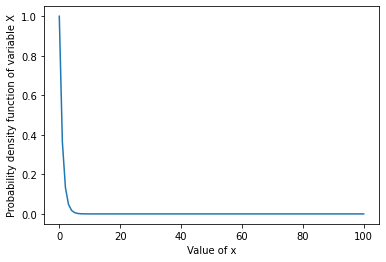
\includegraphics[width=\columnwidth]{solutions/2013/june/42/figures/figure2.png}
%     \caption{P.D.F. of X }
%     \label{june2013-42:june2013-42:fig:fig_label}
% \end{figure}
Let $f_X(x)$ denote the probability distribution function for random variable X.
\begin{align}
f_{X}(x)=
 \begin{cases} 
      \lambda_X  e^{-\lambda_X  x} & x \geq 0 \\
      0 & otherwise
 \end{cases}
\end{align}
Let $f_Y(y)$ denote the probability distribution function for random variable Y.
\begin{align}
f_{Y}(y)=
 \begin{cases} 
      \lambda_Y  e^{-\lambda_Y  y} & y \geq 0 \\
      0 & otherwise
 \end{cases}
 \end{align}
 Let $F_X(x)$ denote the cumulative distribution function for random variable X.
\begin{align}
F_{X}(x)=
 \begin{cases} 
      1-e^{-\lambda_X  x} & x \geq 0 \\
      0 & otherwise
 \end{cases}
\end{align}
Let $F_Y(y)$ denote the cumulative distribution function for random variable Y.
\begin{align}
F_{Y}(y)=
 \begin{cases} 
      1-e^{-\lambda_Y  y} & y \geq 0 \\
      0 & otherwise
 \end{cases}
 \end{align}
\begin{equation}\label{june2013-42:meanx}
    E(X)=\dfrac{1}{\lambda_X}
\end{equation}
\begin{equation}\label{june2013-42:meany}
    E(Y)=\dfrac{1}{\lambda_Y}
\end{equation}
From \ref{june2013-42:meanx} and \ref{june2013-42:meany},
\begin{equation}\label{june2013-42:lambda}
    \lambda_X = \lambda_Y = 1
\end{equation}
\begin{figure}[h]
    \centering
    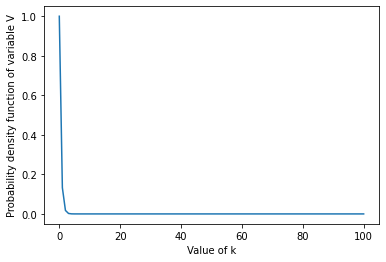
\includegraphics[width=\columnwidth]{solutions/2013/june/42/figures/figure.png}
    \caption{Parallel system}
    \label{june2013-42:fig:fig_label}
\end{figure}
Let Z be a random variable such that $Z=max(X,Y)$
\begin{align}
    P(Z\leq z) &= P(max(X,Y) \leq z)
    \\
    &=P(X\leq z,Y\leq z)
    \\
    &=P(X\leq z) P(Y\leq z)
    \\
    &=(F_X(z)-F_X(0)) (F_Y(z)-F_Y(0))
    \\
    &=1-e^{-(\lambda_X) z}-e^{-(\lambda_Y) z}+e^{-(\lambda_X+\lambda_Y) z}
\end{align}
$P(Z\leq z)$ denotes the probability that the system dies in the first $z$ seconds.\\
\begin{align}
    Expectation &= \int_{0}^{\infty}z \,d(P(Z\leq z))
    \\
\nonumber    &=\int_{0}^{\infty}z(\lambda_Xe^{-(\lambda_X) z}+\lambda_Ye^{-(\lambda_Y) z}\\
&-(\lambda_X+\lambda_Y)e^{-(\lambda_X+\lambda_Y) z}) \,dz
    \\
    &= \dfrac{1}{\lambda_X}+\dfrac{1}{\lambda_Y}-\dfrac{1}{\lambda_X+\lambda_Y}
\end{align}
From \ref{june2013-42:lambda}, 
\begin{equation}
    Expectation=\dfrac{3}{2}
\end{equation}
Therefore, option C correct.


\end{enumerate}